\documentclass{article}
\usepackage{listings}
\usepackage{color}
\usepackage{enumerate}
\definecolor{dkgreen}{rgb}{0,0.6,0}
\definecolor{gray}{rgb}{0.5,0.5,0.5}
\definecolor{mauve}{rgb}{0.58,0,0.82}
\usepackage{lineno}


\lstset{frame=tb,
  language=Haskell,
  aboveskip=3mm,
  belowskip=3mm,
  showstringspaces=false,
  columns=flexible,
  basicstyle={\small\ttfamily},
  keywordstyle=\color{blue},
  commentstyle=\color{dkgreen},
  stringstyle=\color{mauve},
  breaklines=true,
  breakatwhitespace=true,
  tabsize=3,
  numbers=left,
  numbersep=5pt
}
\usepackage[utf8]{inputenc}
\usepackage{enumerate}
\usepackage{graphicx}
\usepackage{hyperref}
\usepackage{wrapfig}

\title{Wlp in Spin}

\author{
Ferdinand van Walree\\
\texttt{3874389}\\
\href{mailto:F.R.vanWalree@students.uu.nl}{F.R.vanWalree@students.uu.nl}
\and
Matthew Swart\\
\texttt{5597250}\\
\href{mailto:m.a.swart@students.uu.nl}{m.a.swart@students.uu.nl}
}
\date{\today}

\usepackage[citestyle=numeric,bibstyle=numeric, sorting=none, backend=bibtex]{biblatex}
\addbibresource{ref.bib}

\begin{document}
\maketitle


\section{Introduction}
This document describes the approach on how we implemented the WLP engine. The engine is written in Haskell. In order to proof the Wlp we use the data.SBV package. We divided the document in 6 section and each of the section explains a particular part of the system. 
To get an impression on how to write GCL in our code, see the following code:
\begin{lstlisting}
{b == 0} a := b - 1 {a == 0}
\end{lstlisting}
 You need to write it like this in our engine:
\begin{lstlisting}
plusExample :: Stmt
plusExample = 
 var [int "a", int "b"]
    [
      assume (i 1 .== ref "b"),
      ref "a" .= ref "b" `minus` i 1,
      assert (ref "a" .== i 0)
    ]
\end{lstlisting}

To see all the possibilities see gcl.hs and examples.hs.

\section{Implementation overview}
This section consist of an overview of all the implemented components. We implemented the following features:
\begin{enumerate}
\item{Base implementation}
\item{Simultaneous assignment}
\item{Array assignments}
\item{Program call}
\end{enumerate}

In the the next part of the document we describes in more detail all of the components listed above. Each of the sections will also contain an example that shows our best work of that particular component. 

\section{Base implementation}
The first implementation is the base implementation. In this part of the engine we created the basic structure. The structure is divided into four components. See figure 1.

\begin{wrapfigure}{r}{0.5\textwidth}
  \begin{center}
    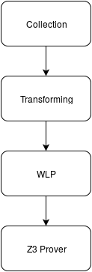
\includegraphics[width=0.20\textwidth]{Architecture1.png}
  \end{center}
  \caption{Structure}
\end{wrapfigure}

\subsection{Collection}
The syntax to represent GCL is defined in \textbf{Attribute.ag}. In \textbf{Collection.ag} we collect all the variables and programs calls. In the collection of the variables we divide vars and refs into separate lists. We do this to distinguish between arrays and integer variable. For example to define an integer variable you need to write: int "a". The program call is explained in chapter 6.

\subsection{Transforming}
The transforming is written in Transformer.hs. In this file we first introduce new fresh variables. We do this by folding over the Statements and Expression. In the folding we keep track of a number, which we add at the end of each variable. If we pattern match on Var, we will increase this number, so that all of the variable of the var will have 1 higher than the previous var type. However, in the forall we also do this. In the transforming we also added array and program calls, but this will be explained later in the document.



\subsection{Verification}
In \textbf{verification.hs} we calculate the WLP. We do this by recursive going over the wlp function. In order to calculate the WLP we use the lemma's of the lecture notes. However, there are some special cases where we had to do more work. In the assign we had modified the Q. The second case is in the while. In the while there are 2 special cases. If the while is provided with an invariant, we need to proof that invariant first. Nevertheless,  we always calculate the wlp, even when the invariant is not correct. If the while does not have an invariant, we calculate a fixpoint. This is explained in 7 Loop reduction.



\subsection{Prover}
The last part of the structure is the Prover. This is written in \textbf{Prover.hs}. In this file we proof the WLP, calculated in the verification. In order to proof the WLP we use the package Data.SBV. The first thing we do to proof is to store the of all the variables its value. This has the possibility to be an int or array. We need to distinguish between these two, so we use two maps to store them. Now that we retrieved all the possible variables, we will  transform our calculate WLP to the correct 

proveImpl :: Expr -> Expr -> IO SBV.ThmResult
mkSymEq :: M.Map String SInteger -> M.Map String (SArray Integer Integer) -> Expr -> Symbolic (Either SInteger (SArray Integer Integer))
mkPred :: M.Map String SInteger -> M.Map String (SArray Integer Integer) -> Expr -> Predicate
mkSymInt :: M.Map String SInteger -> M.Map String (SArray Integer Integer) -> Expr -> Symbolic SInteger
mkInt :: M.Map String SInteger -> M.Map String (SArray Integer Integer) -> (SInteger -> SInteger -> SInteger) -> Expr -> Expr -> Symbolic SInteger


\subsection{Example}
To see what is possible see the following code:
\begin{lstlisting}
s1 :: Stmt
s1 = var [int "x",int "y",int "n"] 
            [ assume (i 0 .<  ref "x") ,
                inv (i 0 .<= ref "x")
                    (while (i 0 .< ref "x")  [(ref "x") .= (ref "x" `minus` i 1) ]),
                ref "y"  .= ref "x",
                assert (ref "y" .== i 0)
            ]
\end{lstlisting}
 
This proofs to QED. However when we modify the assert at line 7 to \textit{(ref "y" .== i 0)}, this results in:
\begin{lstlisting}
Falsifiable. Counter-example:
  x0 = 1 :: Integer
\end{lstlisting}


\section{Simultaneous assignment}
In this section we will explain how we implemented simultaneous assignments. We did this in the tranformer.hs.
\begin{lstlisting}
a := 10
a,b := 1, a + 3
\end{lstlisting} 

Transformed to:
\begin{lstlisting}
a0 := 10
a1 := a0
b1 := b0
a0 := 1
b0 := a1 + 3
\end{lstlisting} 

\section{Array assignment}
This section explains how we implemented array assignments in our system. The first thing we did was modify the grammer.ag to add support for GCL arrays using Haskell. We added the constructor Repby to the Expression. For example to use the following array \textbf{a[i] := 1} you need to write this:
\begin{lstlisting}
ref "a" `repby` ref "i" .= i 1
\end{lstlisting}
Next we had to transform the array assigned to the correct type. See the lemma:
\\
P $\Rightarrow$ Q[1/a[i]]\\
$\{$P$\}$ a[i] := 1 $\{$Q$\}$\\

This is done in Verification.hs. In the function wlp we added an extra patten match at the Assign Stmt to support arrays. When the function is executed with that pattern match we will modify the Q, so that all element that consist of the same variable and index as the array will be replaced by the value of correct value. This means that we will replace the value of the array element with the right Expression.


\paragraph{Proof}
Now that we assigned the correct value in Q. This allows us to verify the correctness of the code. We do this in the Prover.hs. To distinguish between variables and arrays we added an extra map, which got as key the variable name and as value the index. We use this array map to get the correct element to get the SInteger of this array. To get the SInteger of an array we use the function readArray from the Data.SBV package to get the correct element. We now can do the same as a normal assignment, the only difference is that we use readarray instead of sInteger. 

Example:
\begin{lstlisting}
swap :: Stmt
swap = var ["a", "i", "j", "tmp", "c", "b"] 
            [assume ((ref "a" `repby` ref "i" .== ref "b") .&& (ref "a" `repby` ref "j" .== ref "c")), 
            ref "tmp" .=  ref "a" `repby` ref "i",
                ref "a" `repby` ref "i" .=  ref "a" `repby` ref "j",
                ref "a" `repby` ref "j" .=  ref "i",
                assert ((ref "tmp" .== ref "b") .&& (ref "a" `repby` ref "i" .== ref "c") .&& (ref "a" `repby` ref "j" .== ref "b"))
            ]
\end{lstlisting}



\section{Program call}
In this section we explain how we implemented the program call in the WLP Engine. In the transformer.hs we added an extra pattern match to transform the program call to the correct form. See lemma:

\begin{lstlisting}
minind :: Stmt
minind = prog "minind" [int "i", int "N", array "a"] [int "r'", int "i'", int "N'", array "a'"]
         [

              var [int "min", int "r", int "j"]
                [
                ref "j" .= ref "i",
                ref "r" .= ref "i",
                ref "min" .= ref "a" `repby` ref "r",
                 inv (forall "x" (ref "j" .< ref "N" .&& ref "j" .<= ref "i" .&& ref "j" .<= ref "r" .&&
                                (ref "j" .== ref "i" .==> ref "r" .== ref "i") .&&
                                (ref "j" .< ref "i" .==> ref "r" .< ref "i") .&&
                                ref "min" .== ref "a" `repby` ref "r" .&&
                                (ref "j" .<= ref "x" .&& ref "x" .< ref "i" .==> ref "a" `repby` ref "r" .<= ref "a" `repby` ref "x")))
                  (while (ref "i" .< ref "N")
                    [
                      if_then_else (ref "a" `repby` ref "i" .< ref "min")
                        [
                          ref "min" .= ref "a" `repby` ref "i",
                          ref "r" .= ref "i"
                        ]
                        [
                          Skip
                        ],
                      ref "i" .= ref "i" `plus` i 1
                    ]),
                ref "r'" .= ref "r",
                ref "i'" .= ref "i",
                ref "a'" .= ref "a",
                ref "N'" .= ref "N"
                ]
  ]

callMinind :: Stmt
callMinind = var [int "i", int "N", array "a", int "r"] [
        assume (ref "i" .< ref "N"),
        minind,
        pcall "minind" [ref "i", ref "N", ref "a"] [ref "r", ref "i", ref "N", ref "a"],
        assert (forall "x" (ref "i" .<= ref "x" .&& ref "x" .< ref "N" .==> 
                                   (ref "a" `repby` ref "r" .<= ref "a" `repby` ref "x")))
    ] 
\end{lstlisting}


\section{Loop reduction}
This explains how the loop reduction is implemented. In the Verification.hs we added an extra pattern match for a while without an invaraint, which tries to calculate a fixpoint of the While. This is done in the loopReduction function. If the function does not find a fixpoint, we return the w0 calculation. Otherwise we return the fixpoint.\\

while G do S\\
$\{$while$\}^{0}$ = $\neg{g} \Rightarrow Q$\\
$\{$while$\}^{1}$ = (g $\wedge$ wlp s $\{$while$\}^{0}$) $\vee$ ($\neg{g}$ $\wedge$ Q)

For example we have this code:

\begin{lstlisting}
loopExample :: Stmt
loopExample = 
	var [int "y"]
      [
        assume (i 0 .<= ref "y"),
        while (i 0 .< ref "y") [ref "y" .= ref "y" `minus` i 1],
        assert (ref "y" .== i 0)
      ]
\end{lstlisting}
Not sure if need to calculate a loop reduction here.
\section{Relevance work}
Relevant work..
%I think we can delelet this section.%
\section{Conclusion}
Conclusion...


\end{document}
